\documentclass[11pt,xcolor=dvipsnames,presentation]{beamer}

\usepackage{BeamerColor}
\usepackage{etoolbox}

\usepackage[T1]{fontenc}%
\usepackage[utf8]{inputenc}%
\usepackage[main= english,francais]{babel}%
\usepackage{mathtools}

\usepackage{graphicx}%
\usepackage{courier}%
\usepackage{algorithm2e}

\usepackage{url}%
\urlstyle{sf}%

\usepackage{subcaption}%
\usepackage{caption}
\captionsetup[figure]{labelformat=empty}% redefines the caption setup of the figures environment in the beamer class.
\usepackage{tikz}
\usetikzlibrary{positioning}

\usepackage{listings}%

\usepackage{faktor}%

\usepackage{stmaryrd}%

\usepackage[style=verbose,backend=biber]{biblatex}
\addbibresource{biblio.bib}

\newcommand\blfootnote[1]{%
  \begingroup
  \renewcommand\thefootnote{}\footnote{#1}%
  \addtocounter{footnote}{-1}%
  \endgroup
}

%%%%%%%%% Colors of Beamer Layout %%%%%%%%%%%%%
\newcommand{\myorange}{Orange}
\newcommand{\mygreen}{DarkGreen}
\newcommand{\mycyan}{LightSeaGreen}
\newcommand{\myred}{RubineRed}
\newcommand{\myyellow}{Goldenrod}
\newcommand{\myblue}{RoyalBlue}

%%%%%%%%% Begin of Beamer Layout %%%%%%%%%%%%%
\ProcessOptionsBeamer
\usecolortheme{whale}
\usecolortheme[named=\myblue]{structure}
\useinnertheme{rounded}
\useoutertheme{infolines}


\setbeamertemplate{footline}[frame number]
\setbeamertemplate{headline}[default]
\setbeamertemplate{navigation symbols}{}
\setbeamertemplate{itemize items}[circle]
\defbeamertemplate*{headline}{info theme}{}
\defbeamertemplate*{footline}{info theme}{\leavevmode%


  \hbox{%
\begin{beamercolorbox}[wd=.2\paperwidth,ht=2.25ex,dp=1ex,center]{author in head/foot}%
\usebeamerfont{author in head/foot}\insertshortauthor
\end{beamercolorbox}%
\begin{beamercolorbox}[wd=.71\paperwidth,ht=2.25ex,dp=1ex,center]{title in head/foot}%
\usebeamerfont{title in head/foot}\insertsectionhead
\end{beamercolorbox}%
\begin{beamercolorbox}[wd=.09\paperwidth,ht=2.25ex,dp=1ex,right]{section in head/foot}%
\usebeamerfont{section in head/foot}\insertframenumber{}~/~\inserttotalframenumber\hspace*{2ex}
\end{beamercolorbox}
}\vskip0pt}
\setbeamercolor*{block title example}{fg=\myorange}
\AtBeginEnvironment{exampleblock}{\setbeamercolor{itemize item}{fg=\myorange}}
\setbeamercolor*{block title alerted}{fg=\myred}
\AtBeginEnvironment{alertblock}{\setbeamercolor{itemize item}{fg=\myred}}
\setbeamertemplate{footline}[info theme]
\defbeamertemplate{description item}{align left}{\insertdescriptionitem\hfill}


\lstset{%
	basicstyle=\sffamily,%
	columns=fullflexible,%
	language=C++,% % À ajuster dans chaque projet!
	frame=lb,%
	frameround=fftf,%
}%

\sloppy

%\setbeamertemplate{headline}{}%

\setbeamertemplate{navigation symbols}{%
	\insertslidenavigationsymbol%
	% \insertframenavigationsymbol%
	% \insertsubsectionnavigationsymbol%
	% \insertsectionnavigationsymbol%
	% \insertdocnavigationsymbol%
	% \insertbackfindforwardnavigationsymbol%
}

\newcommand{\backupbegin}{
   \newcounter{finalframe}
   \setcounter{finalframe}{\value{framenumber}}
}
\newcommand{\backupend}{
   \setcounter{framenumber}{\value{finalframe}}
}

\newcommand{\Imin}{\ensuremath{\rm{I}^-}\xspace}
\newcommand{\Ipl}{\ensuremath{\rm{I}^+}\xspace}
%\newcommand{\Imove}{\ensuremath{\rm{I}}}
\newcommand{\I}{\ensuremath{\rm{I}}\xspace}
\newcommand{\II}{\ensuremath{\rm{II}}\xspace}
\newcommand{\III}{\ensuremath{\rm{III}}\xspace}
\newcommand{\IImin}{\ensuremath{\rm{II}^-}\xspace}
\newcommand{\IIpl}{{\ensuremath{\rm{II}^+}}\xspace}


\DeclareMathOperator{\defect}{def}
\begin{document}

\title{Parameterized complexity of untangling knots}
\author[Clément Legrand]{Clément Legrand-Duchesne}
\institute{LaBRI, Bordeaux}
%\date{\today}
\date{July 4, 2022}

\begin{frame}
  \titlepage
  \begin{center}
  Joint work with Ashutosh Rai and Martin Tancer.
  \end{center}

\end{frame}

\section*{Knot theory background}

\begin{frame}{Untangling problem}
  \begin{columns}
    \begin{column}{.25\textwidth}
      \centering
      
\includegraphics[width=.5\textwidth]{diagram_example.pdf}
    \end{column}
    \begin{column}{.75\textwidth}
      \centering
      \uncover<2->{
      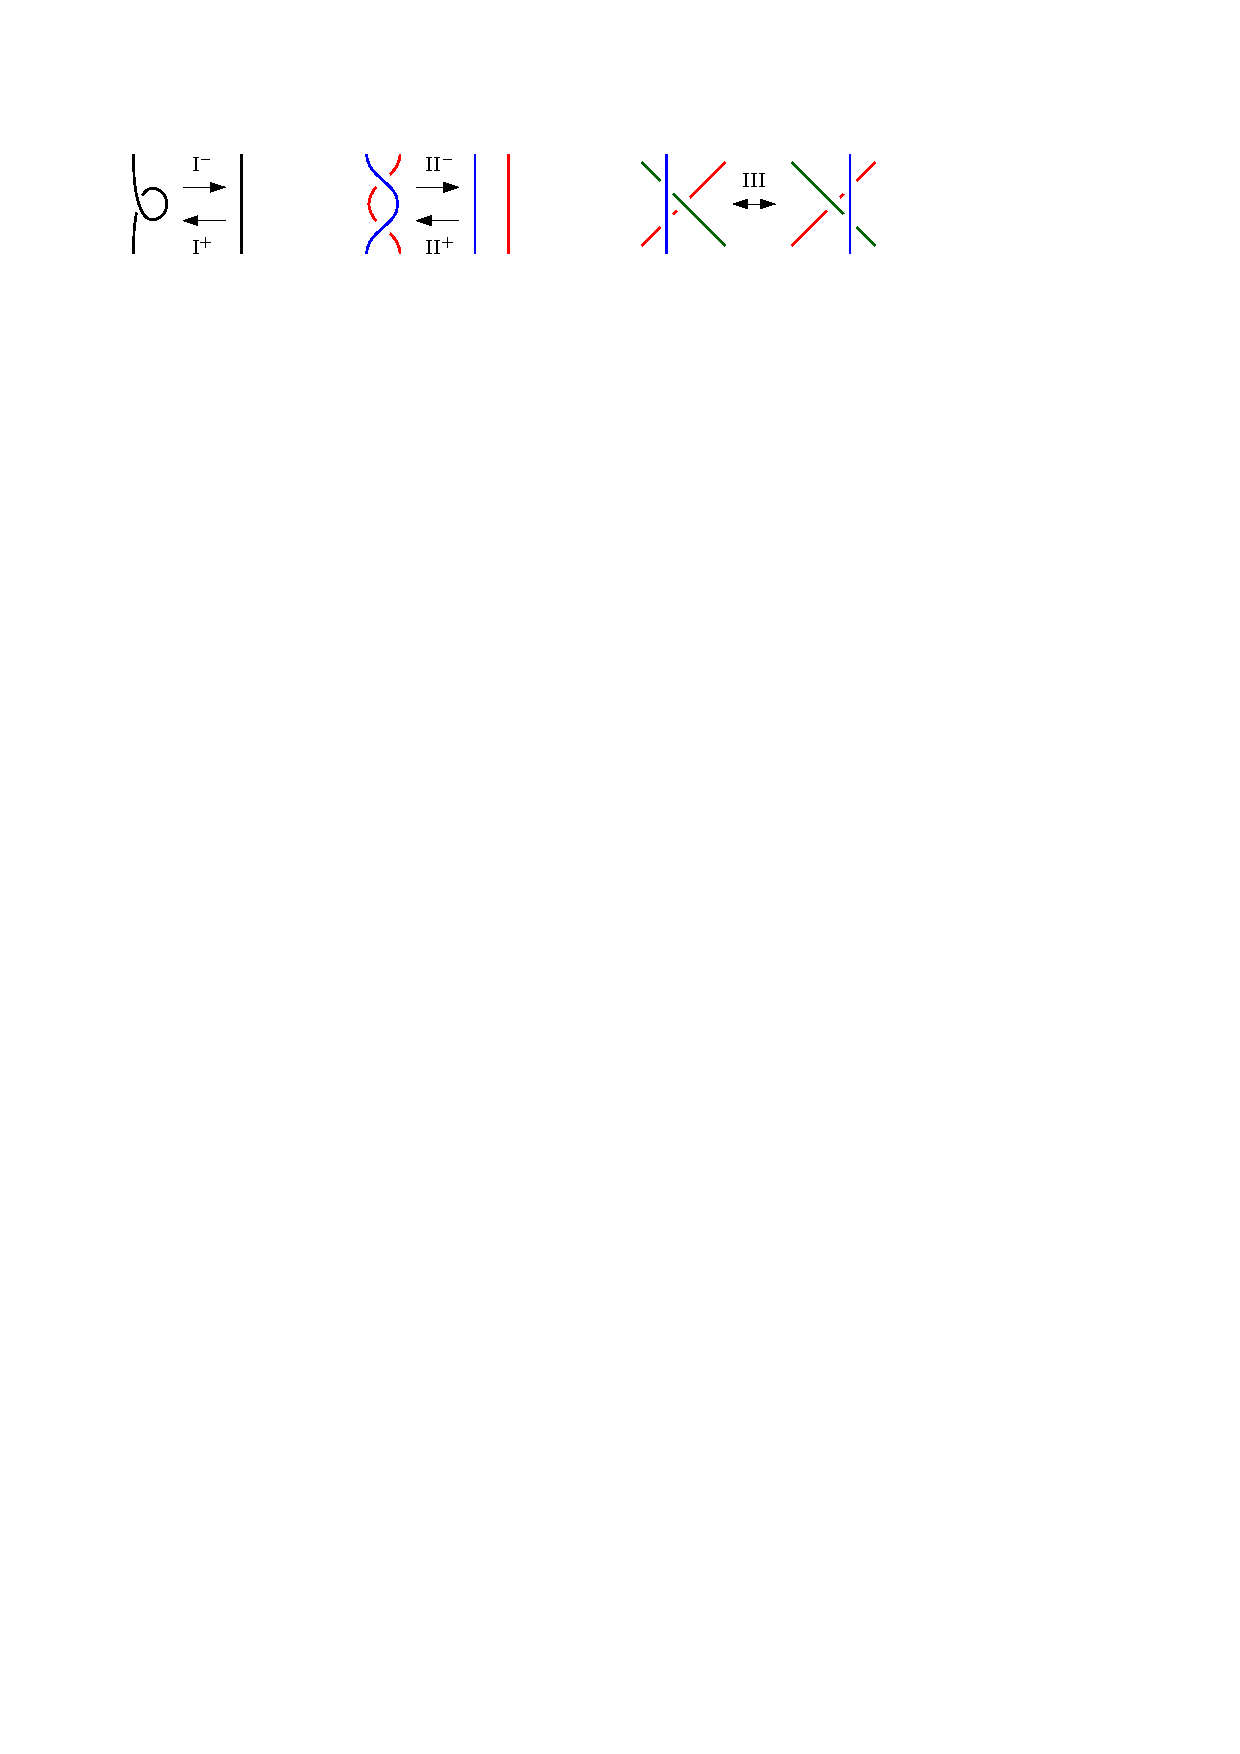
\includegraphics[width=.8\textwidth]{rm.pdf}}
    \end{column}
  \end{columns}

  \uncover<3->{
  \begin{block}{Alexander, Briggs 1926}
    All diagrams of a knot are equivalent up to a series of Reidemeister moves
  \end{block}

  \begin{block}{Lackenby 2015}
    Any diagram of the unknot can be untangled with a polynomial number of moves
  \end{block}

  \begin{block}{de Mesmay, Rieck, Sedgwick and Tancer 2021}
    Shortest Untangling is NP-complete 
  \end{block}}
\end{frame}

\section*{Parameterized complexity background}

\begin{frame}{Main Parameterized complexity classes}
  Idea: express the complexity with regard to the size \textcolor{\myblue}{$n$} and a parameter \textcolor{\myorange}{$k$}

  \vspace{.4cm}
  \begin{center}
  \begin{tikzpicture}
    \pgfmathsetlengthmacro{\yoff}{1cm}%
    \uncover<3->{
    \draw [thick, fill=gray!10] (0,1.7*\yoff) circle[x radius=1.5cm, y
      radius=3cm] ++(0,2.7*\yoff) node (xp) {XP};}

    \uncover<4->{
    \draw [thick, fill=gray!50] (0,1.5*\yoff) circle[x radius=1.3cm, y
      radius=2.6cm] ++(0,2*\yoff) node (wp) {W[P]};
    \node (dots) at (0,2.5*\yoff) {$\vdots$};}

    \uncover<2->{
    \draw [thick, fill=gray!90] (0,0.6*\yoff) circle[x radius=1cm, y
      radius=1.5cm] ++(0,1*\yoff) node{W[2]};
    \draw [thick, fill=gray!130] (0,0.2*\yoff) circle[x radius=.7cm, y
      radius=.9cm] ++(0,0.5*\yoff) node (w1) {W[1]};}
    \node[right = -.4cm of w1] (w1bis) {};

    \draw [thick, fill=gray!170] (0,0) circle[x radius=.5cm, y radius=.5cm] node
    (fpt) {FPT}; 

    \pgfmathsetlengthmacro{\xoff}{1.8cm}%


    \node (legendfpt) at (\xoff,0) {};
    \node[right =.2cm of legendfpt,align=left] (compfpt) {$O(\textcolor{\myorange}{f(k)}\cdot\textcolor{\myblue}{P(n)})$};
    \node[align = left,right] at (3*\xoff, 0.3cm) {SAT with \textcolor{\myorange}{$k$} variables};
    \node[align = left,right] at (3*\xoff, -0.3cm) {vertex cover of size \textcolor{\myorange}{$k$}};
    \draw[thick,->] (legendfpt) -- (fpt);

    \uncover<2->{
      \node (legendw1) at (\xoff,1.5*\yoff) {};
      \node[right =.2cm of legendw1, align=left] (compw1) {defined with \\ combinatorial\\ circuits};
      \node[align = left,right] at (3*\xoff, 1.5*\yoff){independent set of size \textcolor{\myorange}{$k$}};
      \draw[thick,->] (legendw1) -- (w1bis);}

    \uncover<3->{
      \node (legendxp) at (\xoff,4.4*\yoff) {};
      \node[right =.2cm of legendxp, align=left] (compxp) {$O(\textcolor{\myblue}{n}^{\textcolor{\myorange}{f(k)}})$};
      \node[align = left, right] at (3*\xoff, 4.4*\yoff){Non-empty
        intersection\\
      of \textcolor{\myorange}{$k$} tree-automatas};

      \node[right =.2cm of legendxp] {};
      \draw[thick,->] (legendxp) -- (xp);}

    \uncover<4>{
      \node (legendwp) at (\xoff,3*\yoff) {};
      \node[right =.2cm of legendwp, align = left] {non-deterministic : $O(\textcolor{\myorange}{h(k)}\cdot\textcolor{\myblue}{\log(n)})$\\
      + deterministic : $O(\textcolor{\myorange}{f(k)}\cdot\textcolor{\myblue}{P(n)})$};
      \draw[thick,->] (legendwp) -- (wp);}
      
  \end{tikzpicture}
  \end{center}
\end{frame}

\section*{Parameterized complexity of untangling}

\begin{frame}{Choice of the parameter}
  \centering
  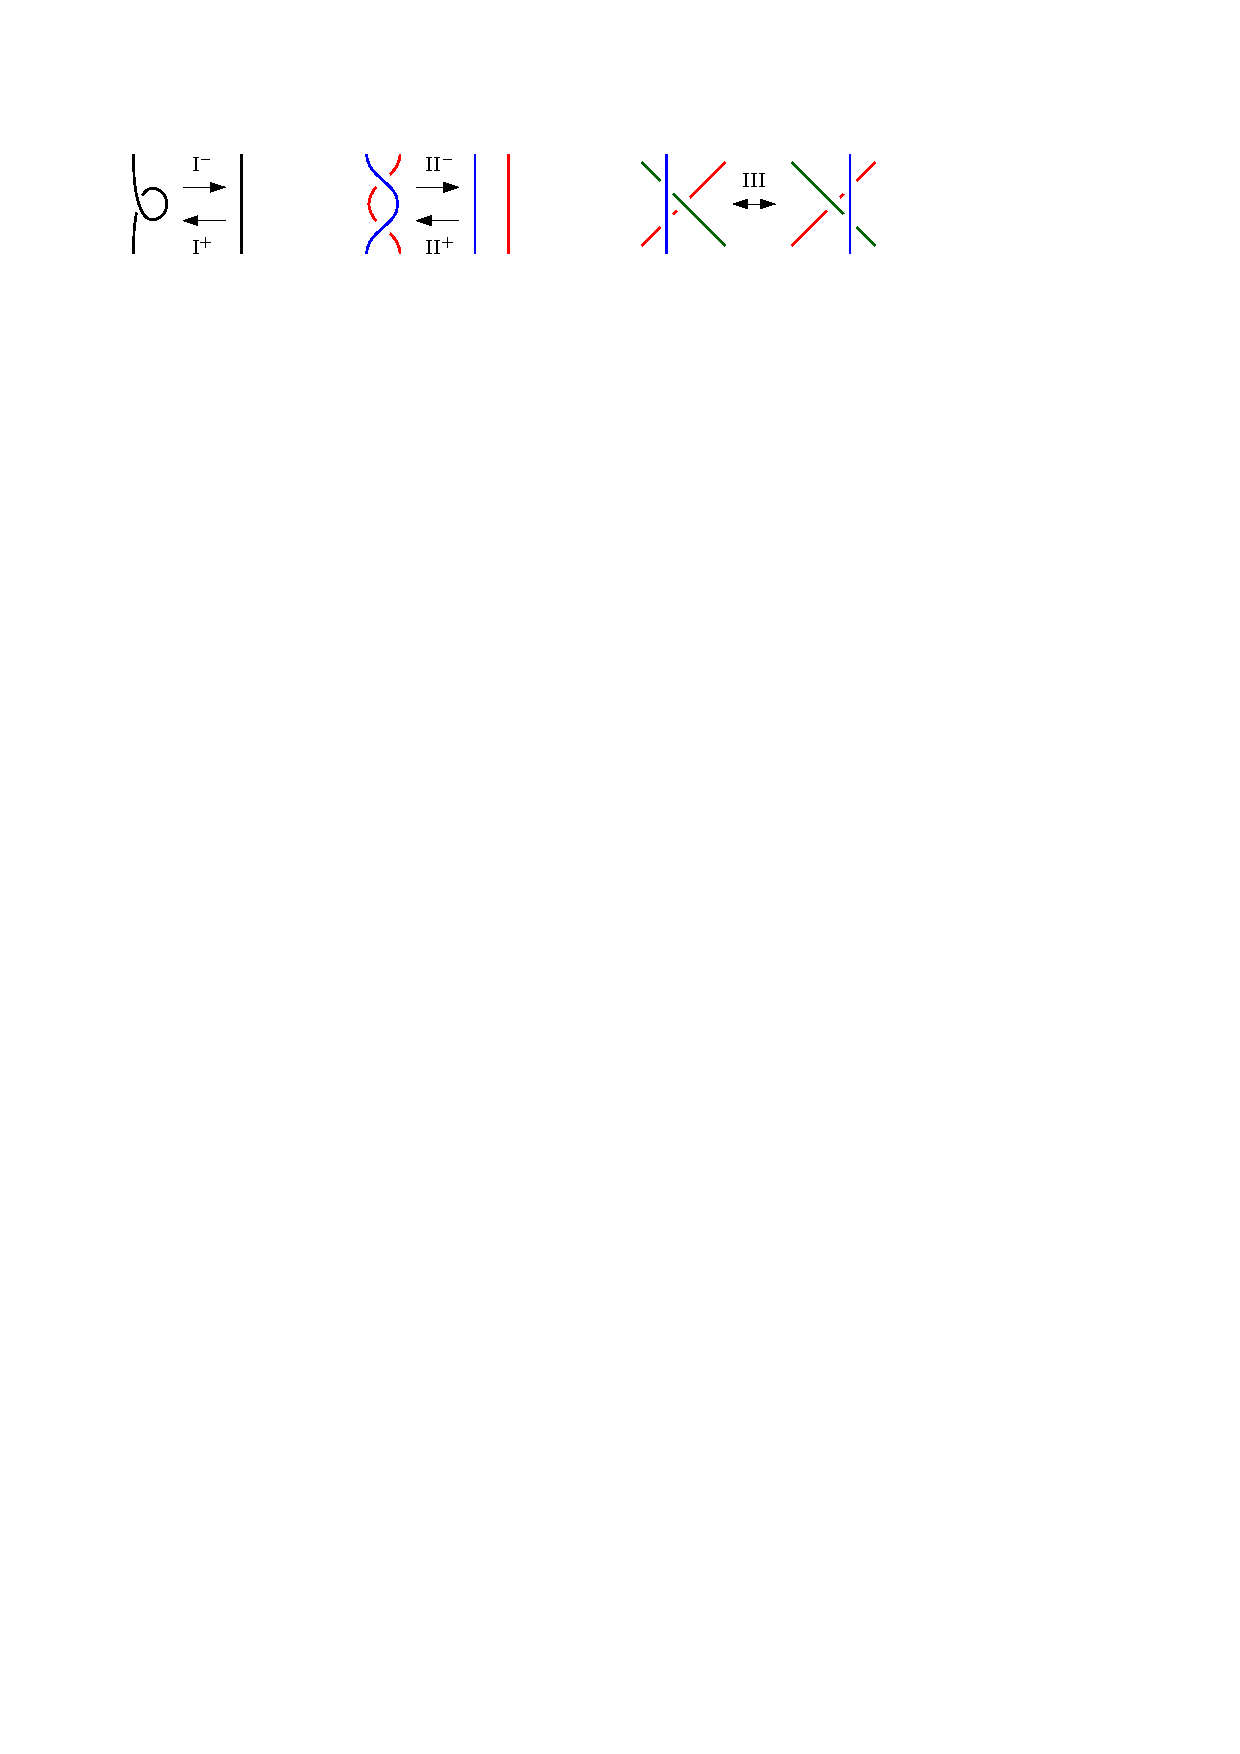
\includegraphics[width=.6\textwidth]{rm.pdf}
  
  \begin{block}{Parameterized by size of the sequence}
    Instances of bounded size $\leadsto$ linear kernel, trivially FPT
  \end{block}

  \uncover<2>{
  \begin{block}{Parameterized by defect}
    $$\defect(S) = 2|S| - n \quad \quad \defect(D) = \min_{S} \defect(S)$$
    \vspace{-.3cm}
    \begin{itemize}
    \item ``counts'' the number non-optimal moves
      $$\defect(S) = \sum_{m \in S} w(m) \quad \quad
      \begin{tabular}{|c|c|c|c|c|c|}
        \hline
        type of move & \IImin & \Imin & \III  & \Ipl & \IIpl \\
        \hline
        weight & 0 & 1 & 2 & 3 & 4\\
        \hline
      \end{tabular}$$
    \item instances of unbounded size
    \item key ingredient in the NP-hardness proof
    \end{itemize}
  \end{block}}
\end{frame}

\begin{frame}{Parameterized complexity of untangling}
  \begin{block}{L., Rai, Tancer 22+}
    Shortest untangling parameterized by defect is W[P]-complete
  \end{block}

  \begin{block}{W[P]- membership}
    Key observation: \IImin can be performed greedily !
  \end{block}
  
  \begin{block}{W[P]-hardness}
    Reduction from Minimum axiom set
  \end{block}
\end{frame}

\section*{Swapping moves and W[P]-membership}

\begin{frame}{\IImin moves can be performed greedily}

  \begin{block}{Untangle$(D,k)$:}
    \vspace{-.4cm}
      \begin{overlayarea}{\linewidth}{0.4\textheight}
      \begin{itemize}
      \item<4-> Non-deterministic choose a set of special crossing $X$
      \item if $k <0$ return NO; if $k = 0$ and $D = U$ return YES;
      \item<2->Deterministic: if there exist a \only<4->{\textbf{greedy} }feasible \IImin move $m$,
        return Untangle$(D(m) , k - w(m))$\\
      \item Non-deterministic: perform any possible Reidemeister move $m$
        \only<4->{\textbf{involving crossings in $X$}} and return Untangle$(D(m),k
        -w(m))$
      \end{itemize}
      \end{overlayarea}
  \end{block}
  
  \begin{overlayarea}{\linewidth}{0.5\textheight}
    \only<3>{
      \vspace{-.8cm}
      \begin{block}{Kauffman, Lambropoulou}
        \centering
        
\includegraphics[width=.3\linewidth]{culprit.pdf}
      \end{block}}
    \only<5>{
      \begin{block}{Key lemma}
        If $S$ untangles $D$ with defect $k$ and there is a greedy feasible
        \IImin move
        $m$, then there exist a sequence of defect $k$, starting by $m$ and
        untangling $D$.
    \end{block}}
  \end{overlayarea}
\end{frame}

\section*{W[P]-hardness}

\begin{frame}{Reduction from mimimum axiom set}
  \begin{block}{FPT-reduction}
    \begin{itemize}
    \item $(x,k) \leadsto (x',k')$ in time $O(f(k)P(|x|))$
    \item $k' \le g(k)$
    \end{itemize}
  \end{block}
  
  \begin{block}{Minimum Axiom Set}
  \begin{description}
  \item[Input] A finite set of variables $\mathcal{S} = \{s_1, \dots s_p\}$\\
    A finite set of relations $\mathcal{R}$ of the form $(T,t)$ with $T \subset
    \mathcal{S}$ and $t \in \mathcal{S}$
  \item[Parameter] $k$
  \item[Ouput] Does there exist $S_0 \subset \mathcal{S}$ of size $k$ such that
    the sequence $$S_{i+1} = S_i \cup \{t | T \subset S_i \text{ with } (T,t)
    \in \mathcal{R}\}$$ verifies $\bigcup_{i=0}^\infty S_i = \mathcal{S}$ ?
  \end{description}
\end{block}
\end{frame}

\begin{frame}{Sketch of the reduction}
  \begin{block}{Brunnian link}
    Non-trivial link that becomes trivial if any of its components is removed
  \end{block}
  \begin{columns}
    \begin{column}{.47\linewidth}
      \centering
      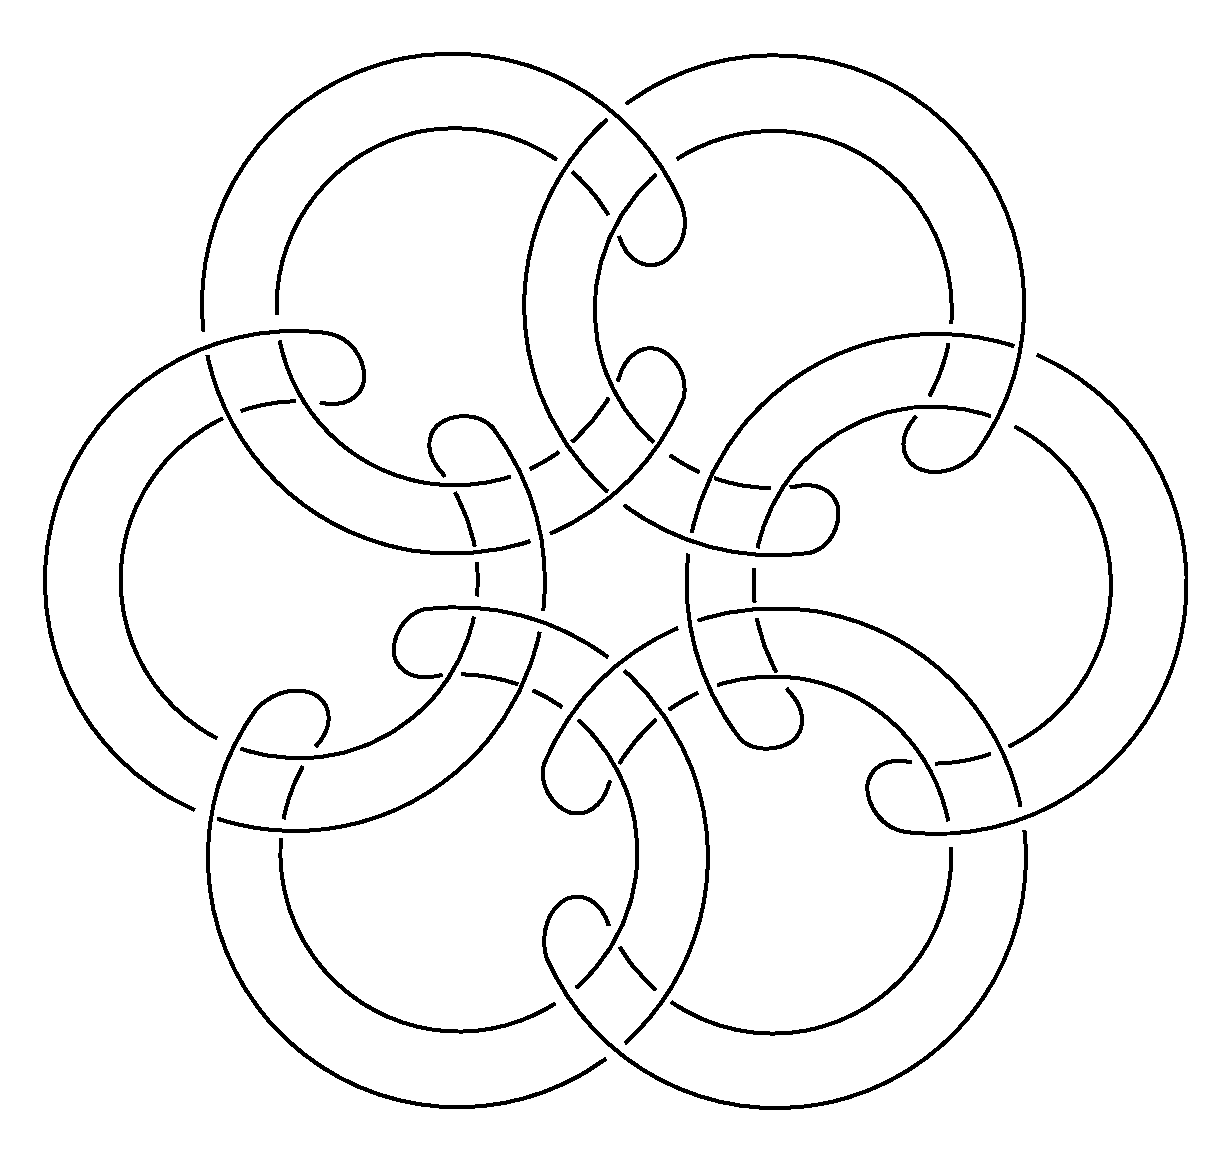
\includegraphics[width=1\linewidth]{rubberband.pdf}
    \end{column}
    \hfill
    \uncover<2->{
    \begin{column}{.52\linewidth}
      \centering
      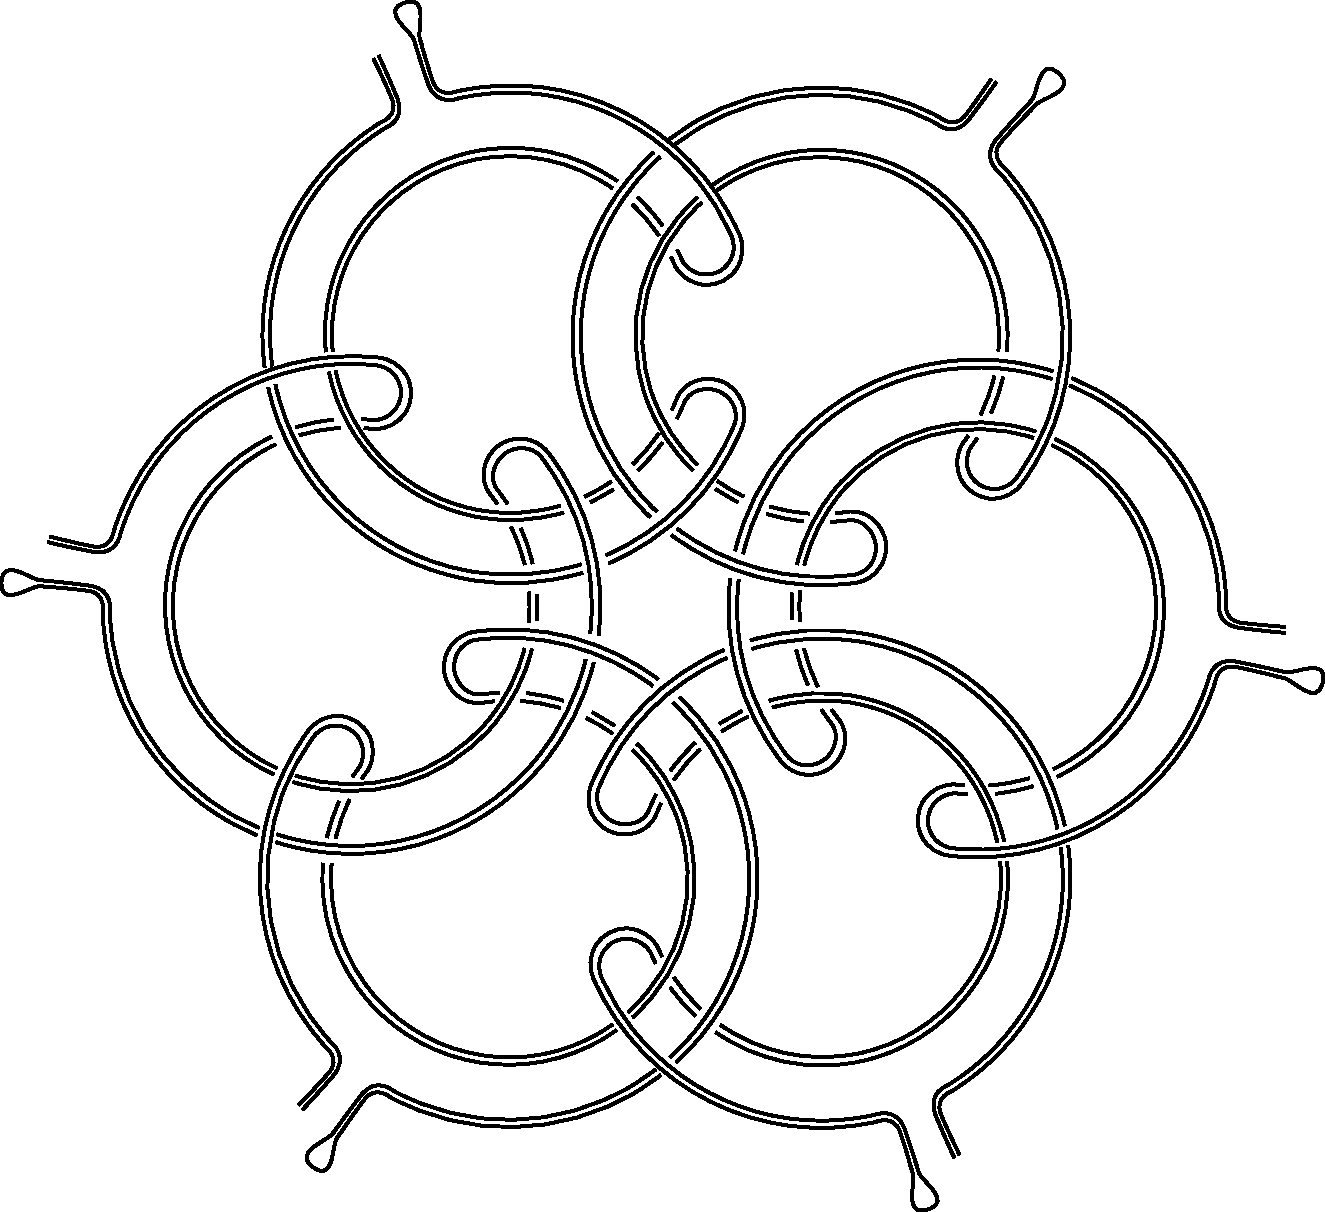
\includegraphics[width=1\linewidth]{rubberband_doubled.pdf}
     \end{column}}
  \end{columns}
\end{frame}

\begin{frame}{Sketch of the reduction}
  \begin{itemize}
  \item One gadget for every variable
  \item In each gadget, twist both ends of the components
  \item Connect
  \end{itemize}
  \centering
 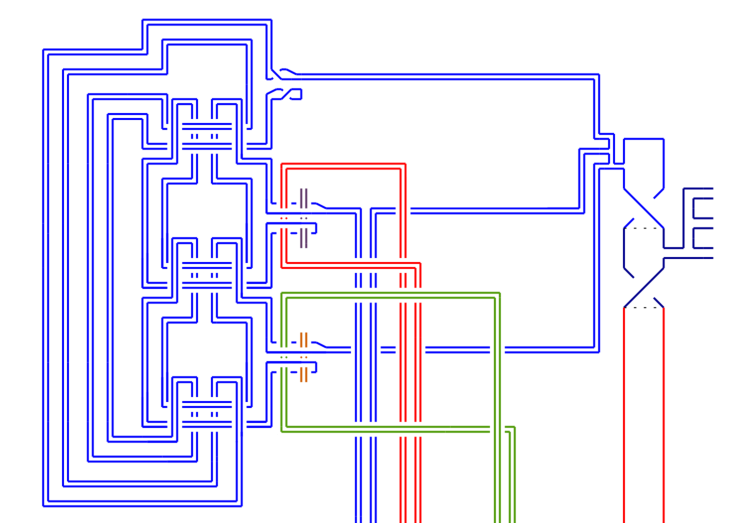
\includegraphics[width=.7\linewidth]{example.pdf} 
\end{frame}


\end{document}
